\documentclass[10pt,a4paper,twocolumn]{article}

\usepackage[margin=0.7in]{geometry}
\usepackage[T1]{fontenc}
\usepackage{lmodern}
\usepackage{microtype}
\usepackage{graphicx}
\usepackage{booktabs}
\usepackage{amsmath}
\usepackage{float}
\usepackage{hyperref}
\usepackage[numbers]{natbib}
\usepackage{enumitem}
\usepackage{xcolor}
\usepackage{fancybox}
\setlist{nosep,leftmargin=*}
\setlength{\columnsep}{0.22in}
\setlength{\parindent}{0pt}
\setlength{\parskip}{0.35em}

\title{\vspace{-1.5em}Coursework Report: Active Learning on a Budget\vspace{-0.75em}}
\author{Ali Alharmoodi}
\date{}

\begin{document}
\maketitle
\vspace{-1.5em}

\noindent\textbf{Code repository:}\\
\url{https://github.com/AliAlharmoodi/MLCW2}

\noindent The accompanying notebook \texttt{Task1\_TPCRP\_CIFAR10.ipynb} contains both the original and modified algorithm implementations for the appendix/code printout requirement.

\section{Introduction}
The paper \emph{Active Learning on a Budget: Opposite Strategies Suit High and Low Budgets} by \citet{hacohen2022active} studies the low-budget active learning regime, where only a very small number of labels can be acquired. Its main claim is that uncertainty-based methods such as margin sampling are weak early on because the classifier is under-trained, while representative and typical samples are more useful. As the budget grows, this preference can reverse.

\section{Methodology and Theory}
The proposed method, TypiClust, is designed for low-budget active learning \citep{hacohen2022active}. Its goal is to select samples that are both \emph{typical} and \emph{diverse}. The method first learns a feature representation of the unlabelled pool using self-supervised learning. For CIFAR-style data, the paper uses SimCLR. It then clusters the learned features and selects one representative point from each chosen cluster.

The method has two main variants. TPCRP performs representation learning followed by a clustering algorithm such as $k$-means. TPC$_{DC}$ uses deep clustering both for representation learning and cluster assignment; in the paper this is done with SCAN. In both cases, the same principle is used:

\begin{enumerate}
    \item Learn feature embeddings for the unlabelled pool.
    \item Partition the embedded points into clusters.
    \item Estimate \emph{typicality} from local density in feature space.
    \item Select the most typical point from each cluster until the budget is exhausted.
\end{enumerate}

Typicality is central to the method. A typical point lies in a dense region of the learned feature space and is therefore likely to be representative. Diversity is enforced through clustering, since sampling from different clusters reduces redundancy.

An important strength of the paper is that this intuition is not only empirical. The authors analyse a two-region mixture model in which the data distribution is split into $R_1$ and $R_2$. Region $R_1$ is easier to learn, $R_2$ is harder, $p$ is the probability mass of $R_1$, and $\alpha>1$ captures the greater difficulty of $R_2$. Writing $E(m)$ for the expected error curve and $E'(m)$ for its derivative, the paper derives the following criterion for which region should be oversampled:
\[
\doublebox{$
\frac{E'(pm)}{E'\bigl(\alpha(1-p)m\bigr)}
\left\{
\begin{array}{l}
> \dfrac{\alpha(1-p)}{p}
\qquad \Longrightarrow \qquad
\textcolor[rgb]{0.35,0.52,0.67}{\text{oversample}}
\\[-2pt]
\qquad\qquad\qquad\qquad\qquad
\textcolor[rgb]{0.35,0.52,0.67}{\text{region } \mathrm{R}_1}
\\[8pt]
< \dfrac{\alpha(1-p)}{p}
\qquad \Longrightarrow \qquad
\textcolor[rgb]{0.35,0.52,0.67}{\text{oversample}}
\\[-2pt]
\qquad\qquad\qquad\qquad\qquad
\textcolor[rgb]{0.35,0.52,0.67}{\text{region } \mathrm{R}_2}
\end{array}
\right.
$}
\]
This condition formalises the paper's phase-transition claim: easier and more typical samples should be preferred early, while harder or more uncertain samples become more useful later.

\section{Modifications}
Our modification keeps the original TPC$_{DC}$ selection rule but changes how cluster-level typicality rankings are reused during acquisition. In the baseline implementation, when a cluster is visited, the method recomputes typicality inside that cluster from scratch, ranks the candidates, and selects the highest-ranked available point. If the cluster is visited again later, the same ranking work is repeated.

The modified version introduces a \emph{refresh-cache} at the cluster level. After a ranking is computed for a cluster, the algorithm reuses that ranking for a limited number of revisits and only refreshes it after enough samples have been removed, or after a fixed number of accesses. In implementation terms, the cache stores a ranked list for each cluster, a pointer to the next candidate, and a lightweight refresh policy that decides when the ranking should be recomputed.

This reduces repeated within-cluster nearest-neighbour computation while trying to stay close to the original TPC$_{DC}$ behaviour.

\section{Results and Statistical Analysis}
The pipeline ran end-to-end and produced CIFAR-10 curves for Margin, and TPC$_{DC}$. The reproduction did not fully match the paper: Margin was best at 20 labels ($+2.44$ over baseline), while TPC$_{DC}$ was negative there ($-1.75$). TPC$_{DC}$ became slightly positive at 50 labels ($+0.84$) and clearly positive at 1000 labels ($+3.16$), but remained below baseline at 100, 200, and 500 labels. These results show a working implementation, but not the strong low-budget TPC$_{DC}$ advantage reported in the paper.

\section{Plots}
The key plot in the paper shows \emph{accuracy difference} relative to the random baseline as a function of the number of labelled examples. This visualises the phase-transition argument directly. At small budgets, the TPC$_{DC}$ curve is above the random and margin baselines, indicating that typicality-based selection is beneficial early. As the budget increases, this advantage decreases.

\begin{figure}[H]
\centering
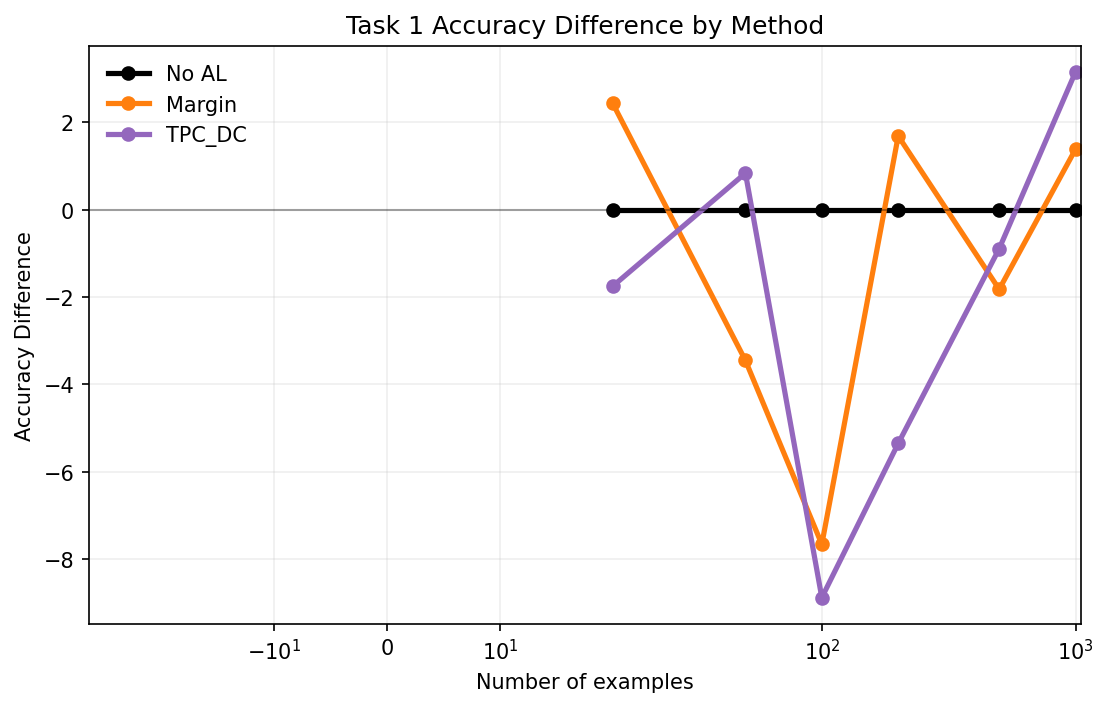
\includegraphics[width=\linewidth]{task1_accuracy_difference.png}
\caption{Reproduced CIFAR-10 accuracy difference plot for No AL, Margin, and TPC$_{DC}$. Positive values indicate improvement over the No AL baseline.}
\end{figure}

\section{Improvement}
The proposed modification was evaluated by comparing the original TPC$_{DC}$ selection routine with the refresh-cache variant while timing only the selection step on fixed cluster assignments. This isolates the effect of the modification from SCAN training and feature extraction.

At 200 labels, the refresh-cache version preserved the same selected set but was slightly slower ($0.96\times$ speedup). At 500 labels, it again preserved the same selected set and reduced runtime from $1.32$s to $0.71$s ($1.86\times$). At 1000 labels, runtime dropped from $1.62$s to $0.48$s ($3.35\times$). Although the selected set no longer matched exactly, the overlap remained 885/1000 samples (88.5\%, Jaccard $0.794$), and 89.6\% of the mismatched samples were replaced by a nearest counterpart from the same cluster. This indicates a useful speed-fidelity tradeoff rather than a qualitatively different acquisition policy.

\begin{figure}[H]
\centering
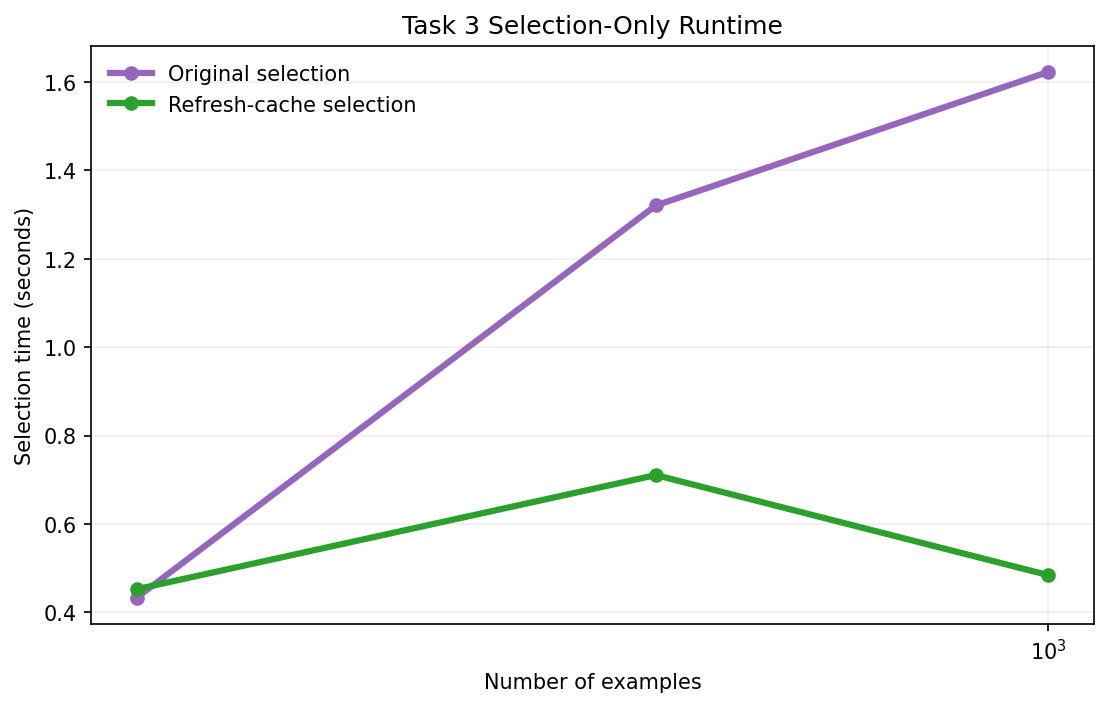
\includegraphics[width=\linewidth]{task3_refresh_cache_timing.png}
\caption{Task 3 selection-only runtime for the original TPC$_{DC}$ routine and the refresh-cache variant.}
\label{fig:task3}
\end{figure}

\section{Conclusion}
In this coursework, the core pipeline was implemented successfully on CIFAR-10, but the reproduced trend only partially matched the paper. The improvement, refresh-cache modification reduced selection time at medium and high budgets while largely preserving the structure of the original selections.

\bibliographystyle{plainnat}
\nocite{hacohen2022active}
\bibliography{references}

\end{document}
